\documentclass[showkeys,reprint,superscriptaddress]{revtex4-2}
%\documentclass[showkeys,preprint]{article}
\usepackage{hyperref}
\hypersetup{colorlinks=true, citecolor=blue, urlcolor=blue, linkcolor=blue}

\usepackage[utf8]{inputenc}
\usepackage{natbib}
\usepackage{graphicx}
\usepackage{amsmath}
\usepackage{lipsum}
\begin{document}
\title{Adiabatic Theory of Resonant Particle Dynamics with Frequency-Chirping Chorus Waves in Inhomogeneous Magnetic Fields}
%Does the adiabaic invariant exists during particle interacting with the frequency chirping wave?
\author{Jiangshan Zheng}
\affiliation{School of Physics, Beihang University, Beijing, 100191, China}
\author{Ge Wang}
%\affiliation{Institute for Fusion Studies, The University of Texas, Austin, Texas 78712, USA}
\affiliation{Center for Plasma Theory and Computation, Madison, Wisconsin 53706, USA}
\author{Bo Li}
\affiliation{School of Physics, Beihang University, Beijing, 100191, China}
\date{\today}

\begin{abstract}
 We present the adiabatic regime for the particles interacting with the frequency chirping waves in the inhomogeneous magnetic field. 
%Based on our previous Hamiltonian formalism \cite{zheng2024}, we give the definition of the adiabatic invariant $\mathcal{I}$.
 Despite the rapid change of the parameters during the interaction, we show that the adiabatic invariant is conserved as long as the particles stay trapped in the reference frame moving with the resonance.
%as long as the particle stay trapped, i.e. the inhomogeniety parameter $\alpha < 0$
%We further 
Assuming the trapped particle distribution as a function of the adiabatic invariant and  the water-bag approximation, we derive an analytic form of the nonlinear current
as a function of 
the inhomogeneous parameter that describes the frequency chirping and inhomogeneities in the background magnetic field.
%We also examine the nonlinear current expression from the  Vlasov hybrid simulations
The nonlinear current expression  is also examined in the  Vlasov hybrid simulations
and the simulation results show that  the nonlinear current can be well described by the adiabatic water bag approximation 
except for the chirping onset stage and the source region where the adiabatic approximation is invalid.
%in most of the simulation domain.
%Our theory and the corresponding numerical method are able to provide high resolution in phase space with affordable computation cost, which is urgently required to reveal the underlying physics of the nonlinear frequency chirping problem.
\end{abstract}
\maketitle

\section{Introduction}
\label{sec:intro}
%preface wave instabilitys with frequency chirping: fusion and magnetoshpere
Wave-particle resonant interactions play an important role  in a wide range of wave instabilities
%, among which the most representative branch is that occurs 
with frequency chirping in fusion and magnetoshperic plasmas.
In the fusion related plasmas, the frequency chirping often appears with the Alfv\'en wave instabilities \cite{chen2016,wang2018,wang2012,wang2012a} and energetic-particle-driven geodesic acoustic modes \cite{wang2013}.
The wave chirping is usually accompanied by fast ion loss and strong radial transport, which is greatly concerned in the fusion studies.
In the planetary magnetosphere, there exists the chorus wave, which is a peculiar electromagnetic emission with frequency sweeping in the whistler-mode range of frequencies \cite{helliwell1965whistlers,burtis_magnetospheric_1976,tsurutani_postmidnight_1974}. 
The chirping behavior similar to the magnetospheric chorus has also been studied recently in the laboratory plasmas \cite{vancompernolle2015,saitoh2024}.
The chorus waves  play a critical role in the electron acceleration   in the Van Allen radiation belts \cite{horne_wave_2005,thorne_rapid_2013,reeves_electron_2013} and the pulsating aurora  and diffuse auroral precipitation \cite{nishimura_identifying_2010,kasahara_pulsating_2018,thorne_scattering_2010}.
The chorus emission is also related to 
 %which have received a significant research interest, such as in 
 the studies of the superradiance in free-electron lasers \cite{zonca_nonlinear_2021, soto-chavez2012}.

%1. The wave particle interaction as pendulum Hamiltonain Albert
The physics of the chorus wave in essence are the nonlinear wave-particle interactions \cite{oneil1971,oneil1972} between the resonant trapped electrons and the whistler waves \cite{omura_theory_2008, an2019}.
The Hamiltonian treatment of a particle nearly resonant with a monochromatic whistler wave in the inhomogeneous magnetic field has been extensively studied \cite{albert1993,albert2021}.
The particle dynamics can be described by a modified pendulum Hamiltonian, where the trapped particles feel both the wave restoring force and the background drag force related to the frequency variation and magnetic field gradient \cite{zheng2024,tao_trap-release-amplify_2021}.

%What is different for the chirping wave interaction, and what changes
It is worth noting that the parameters in the Hamiltonian are changing as the frequency varying together with the inhomogeneous magnetic field.
Alike to the pendulum system, if the variation of the parameters are slow compare to the trapped particle bounce motion, then the system is adiabatic and there exists an adiabatic invariant associated with the bounce motion.
%adiabaitic: the definiation and judge know the adiabaticity is of imporatant to understand and simplify the question
%argument for the interaction regime and adiabatic, it should not be adiabatic: tao and Bierwage
However, recently studies state that for the chorus frequency chirping problem, the nonlinear chirping timescale $\tau_{nl}$ is comparable to the bounce period $\tau_{b}$. Thus, the interaction is nonadiabatic \cite{tao2017a,tao2017b}. 
%0413 + motivation
However, the judgement on whether the resonance particle go through an adiabatic motion just compare the chirping and bounce scale is too rough.
Firstly, the adiabatic invariant for the trapped particle resonantly interacts with chirping chorus wave in the magnetosphere have never been clear defined, not to mention the violation of such.
Besides, during the triggering and propagation of chorus wave, the particle endures multiple phases of wave-particle interactions depending on the location and time stage of the interaction.
In the early phase of chirping \cite{bierwage2021}, the adiabatic bounce motion does not valid since the trapped have yet to be established.
Also in the wave triggering region, there usually accompany by particle releasing \cite{tao_trap-release-amplify_2021} and fast wave variation, which is also a nonadiabatic process.
However, there also exists a stable trapped behavior \cite{zheng2024} in the propagation region of the chorus off the magnetic equator, where the aidabaticity is not well understand in current studies. 
%we we have done, first: frame of reference, then definition of I
%Understanding the dynamics during the entire wave-particle interaction process
Revealing the restrict criterion for the particle adiabaticity is of great importance.
Not only does it help us to distinguish the key stages of the interaction and understand how the dynamics shift in between, it also provides additional approximations that can be applied to simplify and solve the chorus evolution in the propagation region.

The test particle methods \cite{huanghua_test_ptc,omura_test_ptc,tao_test_ptc} provides an intuitive way to study the particle dynamics under the wave field.
However, the conventional studies usually manage the particles' dynamics in the laboratory reference frame,
%people would see fast varying particle and wave phase, There exists fast varing phase in the interaction Hamiltonian 
in which, the wave vector undergoes accelerated rotation due to frequency chirping and the Hamiltonian involves a fast varying phase term in the wave-particle interaction part. 
Thus, it is hard to tell the adiabaticity in such description.
%However, resonance could obtain ....
However, if we reconsider the interaction on a reference frame that perfectly follows the resonance, i.e., moving in-time with the chirping wave that traps the resonant particle, we would observe no chirping at all. Thus, the fast-varying scale is mitigated and a particle can be regarded as adiabatic as long as it remains trapped. Only the particle near the separatrix region suffers a nonadiabatic motion, as pointed in previous studies \cite{CARY1989287}.

In our previous work, we have developed a novel Hamiltonian theory \cite{zheng2024}. 
Harnessing the local resonance frame of reference, we derived the reduced Hamiltonian that describes the interaction of the particle with the slowly varying envelope.
With a further restriction to the onset stage of the chirping, we have constructed a corresponding $\delta f$ Vlasov simulation method and successful obtained the generation of chirping chorus wave.
Note that, since the background magnetic field can strongly affect the wave-particle interaction process \cite{wu2023,wu_controlling_2020}, our simulation is carried with real Earth dipole field configuration.
The chirping rate and amplitude are well agreement with satellite observation \cite{cully_observational_2011} and PIC simulations with real field parameters \cite{katoh2016}.
%Also, since we choose a static frame that follow the start point of the chirping instead of tracking the chirping with time, the simulation obtains the chirping effect as a slowly varying modulation on the wave envelope. 
The simulated self-consistent slowly varying wave envelope can be readily applied to perform a test particle simulation to study the particle dynamics in a new angle of view, different with conventional test particle methods. 

In this work, we examine the adiabaticity by the test particle simulation and derive the nonlinear current with adiabatic approximation for 
the magnetospheric chorus.
We introduce a canonical transformation that shifts the static frame to a time-independent reference frame which follows with the real time chirping wave in the Vlasov simulation.
For the interaction of chorus waves and energetic electrons,
we solve the Hamilton's equations and calculate the adiabatic invariant from the test particle simulations.
The energetic electrons move opposite to the motion of the chorus wave packet through several distinct regions with different physical properties.
We show that the adiabaticity can be completely different in the different reference frames and in the different regions  along the Earth's dipole magnetic fields. 
In the resonance frame,  the adiabatic invariant is preserved in the most of the  downstream region, where the   chorus waves  propagate with frequency chirping and grow in amplitudes.
As the energetic electrons approach the equator
where the chorus waves are triggered with initial small amplitudes,
the adiabaticity  is no longer valid in the equator and the upstream region  due to the particle releasing.
From the adiabatic invariant, we further obtain a reduced  form of the energetic trapped particle current.
We verify the adiabatic approximation from the nonlinear current calculated in the Vlasov simulation and show that the adiabatic regime is valid in the most of the wave propagation region, except in the source regions where the wave is generated from.

%We organize our 
The paper is organized as follows. In section~\ref{sec:theory}, we review the Hamiltonian theory in the resonance reference frame. In section~\ref{sec:dis},  
the adiabaticity 
is examined by the test particle simulation and  the nonlinear current 
is derived with adiabatic approximation. Finally, the summary is presented in section~\ref{sec:conc}.


\section{ Hamiltonian theory}
\label{sec:theory}
In the previous work, the Hamiltonian for the resonant electrons in the frame of reference moving with the local resonance is derived by the canonical transformation \cite{zheng2024}.
The wave-particle interaction is studied on discrete local spatial cells, and the phase space is described by new canonical coordinates ($\xi$, $\Omega$), 
%\begin{equation}
%    \begin{aligned}
%    \xi &=  \varphi - \phi_f~,
%    \\
%    \Omega &= \frac{p_\parallel}{k}-\Pi~,
%    \end{aligned}
%\end{equation}
%where $\Pi = (\omega - \omega_{ce})/k^2$. 
For each cell at a position $s_i$ along the magnetic field, $\xi$, $\Omega$ phase space is decoupled in the original Hamiltonian, and in our hybrid Vlasov simulation \cite{zheng2024,zheng2023b}, the phase flow for the onset of chorus is considered separately with the following Hamiltonian
\begin{equation}\label{eq.H_lab}
    K = \frac{k_l^2\Omega^2}{2} + \mathcal{R}\left(\frac{\omega_b^2}{k_l^2} (e^{-\imath \xi} + \alpha \cdot \xi) \right)~,
\end{equation}
where $\mathcal{R}$ denotes taking the real part, 
\begin{equation}
    \omega_b^2 = \sqrt{2\omega_{ce}(\mathcal{J}+\Pi+\Omega)}k_l^2 a(s_i,t)
\end{equation}
 is the bounce frequency, and 
\begin{equation}\label{eq.alpold}
   \alpha  = \frac{k_l}{\omega_b^2}(\mathcal{J} - \frac{\Pi}{2}) \frac{d\omega_{ce}}{ds}~,
\end{equation}
is the inhomogeneous parameter that describes the frequency chirping and inhomogeneities in the background magnetic field.
Other coordinates and variables such as the canonical momentum $\mathcal{J}$, gyro frequency $\omega_{ce}$, and parameter $\Pi$ are determined from on each local cell \cite{zheng2024,zheng2023b}.
A contour plot of the Hamiltonian is given in Fig. \ref{fig.Hamcontour}
\begin{figure}
    \centering
    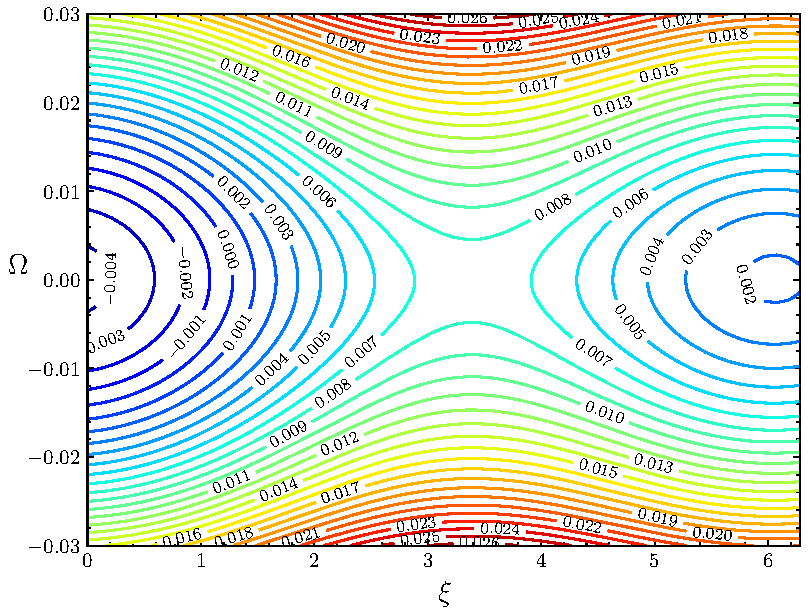
\includegraphics[scale=0.5]{img/Hamcontour.pdf}
    \caption{The contour plot of Hamiltonian in Eq. (\ref{eq.H_lab}) using fixed $\mathcal{J}, a, \Pi$ parameters. 
    \label{fig.Hamcontour}
    }
\end{figure}

Note that we have fixed the reference frame on the most unstable wave with frequency $\omega_l$ and wave number $k_l$,
which corresponds to the onset of the chirping wave.
The reference frame we choose is determined from fixed frequency and wave number which does not change with time, thus we refer such reference frame as the static resonance frame hereafter. 
The simulated wave vector $a$ becomes a complex number with an additional phase $\delta \phi$ due to the static frame can not exactly follow the real time resonance. Therefore we take the real part in the wave-particle interaction term in the above Hamiltonian.
The complex wave vector field $a$ can be written as 
\begin{equation}
    a(s,t) = |a(s,t)| \cdot e^{\imath \delta \phi(s,t)}~,
\end{equation}
where $\delta \phi$ can be regarded as a modulation on the wave envelope, as shown in Fig. \ref{fig.aanda}.

%\begin{equation}\label{eq.cell_j}
%    (\omega_l - \omega_{ce})\mathcal{J} +  \frac{(\omega_l - \omega_{ce})^2}{2k_l^2} = \mathrm{Const.}
%\end{equation}
%Since we consider the parallel propagating wave, 
%%the cell is aligned with the field line, and 
%the reference frame moves according to the 
%resonance 
%velocity,
%\begin{equation}\label{eq.cell_s}
%    \frac{d s_i}{d t} = \frac{\omega_l-\omega_{ce}}{k_l}~.
%\end{equation}

\begin{figure}
    \centering
    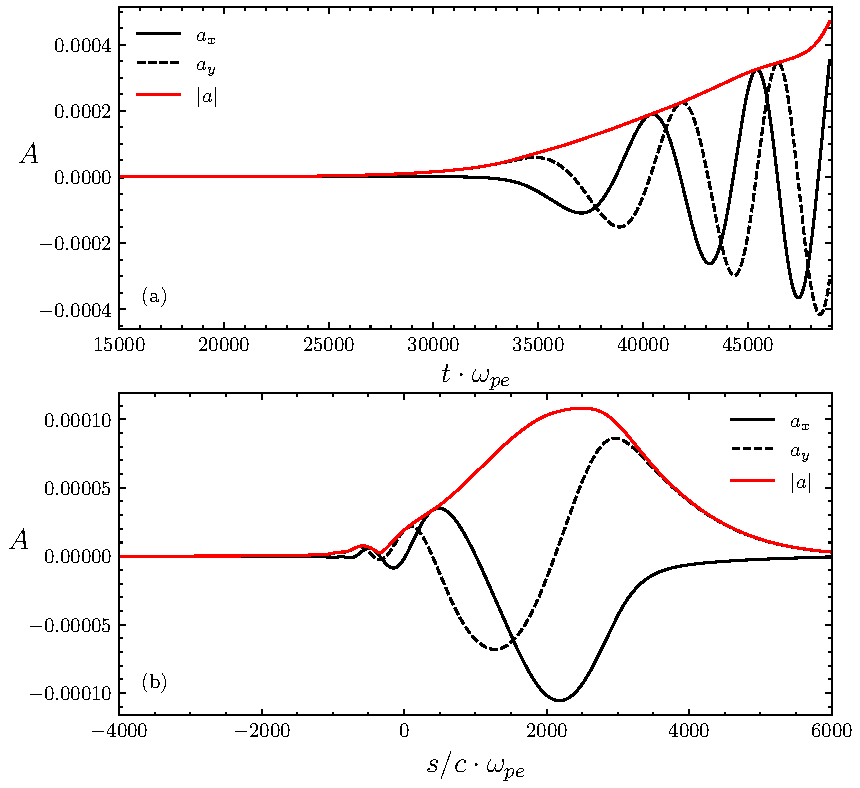
\includegraphics[scale=0.5]{img/aanda.pdf}
    \caption{(a) Time evolution and (b) spatial distribution of the orthogonal components of vector potential, $a_x$ and $a_y$, and the amplitude $|a|$ in the simulation.
    \label{fig.aanda}
    }
\end{figure}

%In other word, $a$ is a complex number and so does $\omega_b$.

%particle trajectory
The varying phase $\delta \phi(s,t)$ indicates the acceleration of trapped particles along $\Omega$ momentum dimension in phase space.
Combining the calculated wave fields  in the Vlasov simulation \cite{zheng2024}, we solve the equations of motion using the Hamiltonian in Eq. (\ref{eq.H_lab}) and show the particle phase space trajectories in Fig. \ref{fig.phaseflow}(a). 
In the static resonance frame, trapped particles do not have a closed phase space trajectory and  their angle variable $\xi$  is shifting and matching with the wave phase $\delta \phi$ along its trajectory, as illustrated in Fig. \ref{fig.phaseflow}(b). This is in accordance with the phase locking condition \cite{tao_trap-release-amplify_2021}.
Their momenta, as shown in Fig. \ref{fig.phaseflow}(c), are also accelerating upwards along $\Omega$ dimension due to the rising tone frequency chirping.

\begin{figure}
    \centering
    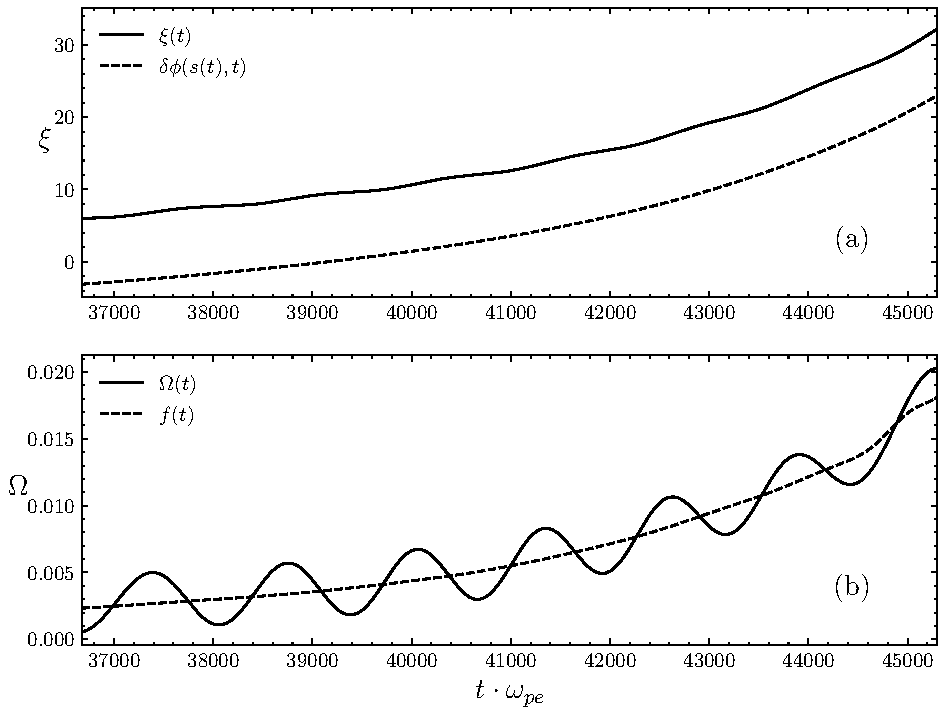
\includegraphics[scale=0.5]{img/phaseflow.pdf}
    \caption{(a) Phase space trajectories of  test particles with initial angle $\xi = 5$ sampled in $\Omega \in [-0.01,0.01]$, (b) typical variation of angle coordinate $\xi$ of a test particle and the cooresponding wave phase $\delta \phi$ along its trajectory. (c) the corresponding variation of particle momentum $\Omega$ with time. The dashed line denotes Eq. (\ref{eq.ft}).
    \label{fig.phaseflow}
    }
\end{figure}

Since the wave phase $\delta \phi$ can be calculated from the Vlasov simulation
 \cite{zheng2024}, we can construct a canonical transformation to shift the static resonance frame back to the real-time resonance frame of reference.
To do so, the new angle variable and momentum  take the following forms \cite{berk1999},
\begin{equation}
    \begin{aligned}
        Q &= \xi - \delta \phi(s(t),t)~,
        \\
        P & = \Omega - f(t)~,
    \end{aligned}
\end{equation}
where $f(t)$ is a time dependent function to be determined.
The above transformation corresponds to a type-2 generating function
\begin{equation}
    F_2(\xi,P,t) = (\xi - \delta \phi) \cdot P + \xi \cdot f(t)
\end{equation}
and the corresponding new Hamiltonian $K^\prime$ is
\begin{equation}
    \begin{aligned}
        K^\prime & = K + \frac{\partial F_2}{\partial t}
        \\
        & = \frac{k_l^2}{2}(P+f(t))^2 + \sqrt{2\omega_{ce}(\mathcal{J}+P+f(t)+\Pi)} \cdot |a|\cos(Q) 
        \\
        & + ((\frac{1}{k_l}(\mathcal{J} - \frac{\Pi}{2}) \frac{d\omega_{ce}}{ds})  +\frac{d f(t)}{d t} )\cdot(Q + \delta \phi)  - \frac{d \delta \phi}{d t} P ~. 
        \end{aligned}
\end{equation}
In addition,  the first order term with respect to $P$ 
should be eliminated
in the above Hamiltonian, which determines $f(t)$ as
\begin{equation}\label{eq.ft}
    \begin{aligned}
    f(t) & = - \frac{1}{k_l^2} \frac{d \delta \phi}{d t}  &= \frac{\delta \omega - v_r \delta k}{k_l^2}~.
    \end{aligned}
\end{equation} 
Note that the exact time derivative is evaluated along the particle trajectory, $d/dt = \partial/\partial t + v_r \partial /\partial s$ with $\delta \omega  \equiv \partial \delta \phi/\partial t$ and $\delta k  \equiv -\partial \delta \phi/\partial s$.
We can examine that $f(t)$ is the first order variation of $\Omega(\omega,k)$ due to the chirping frequency $\delta \omega$, and the variation of wave number $\delta k$.
The expression also agrees with the change of $\Omega$ in the test particle results shown in Fig. \ref{fig.phaseflow}(c).
%\begin{equation}
%    \begin{aligned}
%    \delta \omega & \equiv \frac{\partial \delta \phi}{\partial t}~,
%    \\
%    \delta k & \equiv -\frac{\partial \delta \phi}{\partial s}~,
%    \end{aligned}
%\end{equation}
For the derivative of $f(t)$, we only keep the term up to the first order, which gives
\begin{equation}
    \frac{d f(t)}{d t} \simeq \frac{1}{k_l^2}(\frac{\partial \delta \omega}{\partial t} + 2 v_r \frac{\partial \delta \omega}{\partial s} + \frac{3}{2}v_r\frac{\delta k}{k_l} \frac{d \omega_{ce}}{d s}  ).
\end{equation}
Finally, the new Hamiltonian takes the following form 
\begin{equation}\label{eq.H_frame}
    K^\prime = \frac{k_l^2 P^2}{2} + \frac{\omega_b^2}{k_l^2} (\cos Q + \alpha \cdot Q)~,
\end{equation}
where
\begin{equation}
    \omega_b^2 = \sqrt{2\omega_{ce}(\mathcal{J}+P+f(t)+\Pi)} k_l^2 |a|
\end{equation}
and we have a new $\alpha$
\begin{equation}\label{eq.alpnew}
    \begin{aligned}
    \frac{\omega_b^2}{k_l^2}\alpha & = \frac{1}{k_l}\left(\mathcal{J} - \frac{\Pi}{2}\right) \frac{d\omega_{ce}}{ds} \\
    & + \frac{1}{k_l^2}\left(\frac{\partial \delta \omega}{\partial t} + 2 v_r \frac{\partial \delta \omega}{\partial s} + \frac{3}{2}v_r\frac{\delta k}{k_l} \frac{d \omega_{ce}}{d s}\right)~.
    \end{aligned}
\end{equation}
The additional terms compared to Eq. (\ref{eq.alpold}) first order correction related to frequency chirping and wave number variation.

\begin{figure}
    \centering
    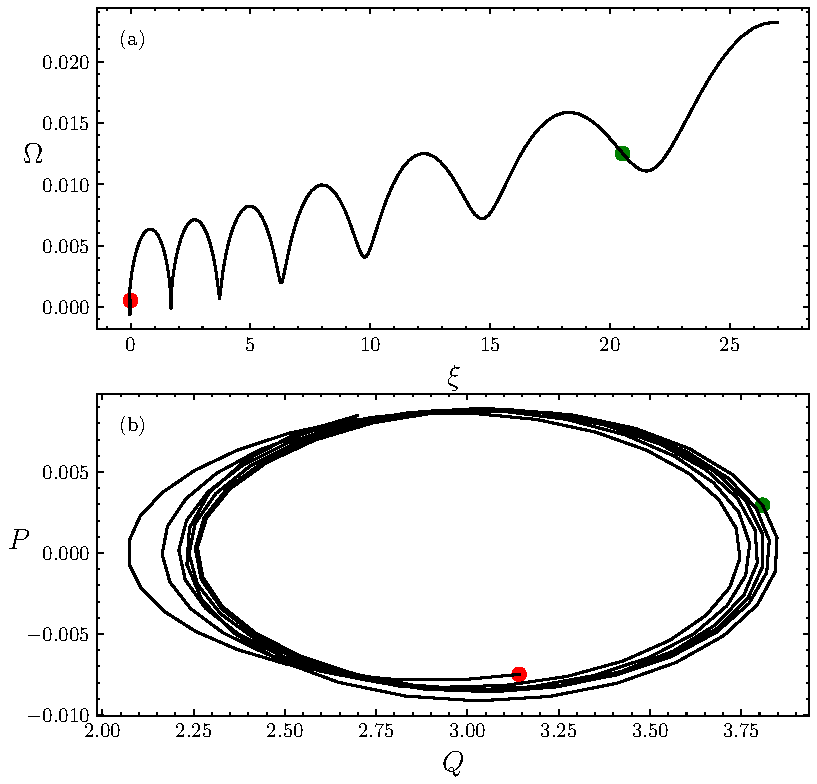
\includegraphics[scale=0.5]{img/Trajectory.pdf}
    \caption{Phase space trajectory of a test particle from $s=700$ at $t=750$ to $s=520$ at $t=930$ (a)  in the static resonance frame and (b)  in the real-time resonance frame. The red dot denotes the start point, and the green dot denotes $t=910$.
    \label{fig.traj}
    }
\end{figure}
%Using the wave data from our Vlasov simualtion, we show the contour plot both of the Hamiltonian (\ref{eq.H_lab}) and the modified Hamiltonian (\ref{eq.H_frame}) in Fig. \ref{fig.Hamcontour}. Due to the $\alpha$/$drg$ term in the Hamiltonian, the trapped region is enclosed between a saddle point  and a C point.
Using the new Hamiltonian, we are able to consider the particle dynamics in real-time resonance frame of reference.
To show the differences, we choose a test particle initially  at the resonance center and calculate its phase space trajectories in the different reference frames in  Fig. \ref{fig.traj}. 
%It can be found that 
In the static  resonance frame, the particle suffers a rapid change in $\Omega$ for each bounce in accordance with  Fig. \ref{fig.phaseflow}(a).
In contrast, there exists only a slight change when we track the particle in the real-time resonance frame, which demonstrates the effectiveness of the canonical transformation.




\section{Adiabatic approximation}
\label{sec:dis}
%\subsection{Adiabatic invariant}
%the adiabatic invariant 
For the resonant electrons trapped by the slowly varying wave envelope and circling around in the phase space,  the adiabatic invariant is defined as
%at a given $s_i$,
\begin{equation}\label{eq.def_I}
    \mathcal{I} = \frac{1}{2\pi} \oint \Omega(H,\xi,t) \mathrm{d} \xi~,
\end{equation}
where $\Omega$ is an implicit function of the Hamiltonian $H$.
%From the above-mentioned
Using the Hamiltonian (\ref{eq.H_lab}) and (\ref{eq.H_frame}), 
%combining the equation of the moving frame along magnetic field line, 
we can numerically calculate the adiabatic invariant $\mathcal{I}$  in the static and moving resonance frames, respectively.

%verify I is invariant
%for different alpha, if the particle remain trapped...
%To do so, we first iterate the phase space flow with time step $\Delta T$ for one fixed $K_i$ at a given $s_i$ and the corresponding background parameters. 
%Then we push the particle to the next location along the field line. 
%For the deeply trapped particle, we just push the particle to the adjacent cell, which is competitive with our Vlasov simulation.
%At new location, we again trace the phase flow with updated background parameter, wave field and new $K_i$.
%By iteratively following the field lines and tracing in phase space, we can construct a continuous trajectory for a particle.

For each temporospatial location, with fixed background and wave parameters, we are able to complete a closed trajectory if the particle stay trapped in the wave field.  
The area of the enclosed loop is actually the phase space integral $\mathcal{I}$.
%Here, , to illustrate the adiabatic invariant, we calculate the closed phase trajectories with parameter at the initial and at the $s=540$, $t=910$ location.
In the static frame, it is clear that the area changes significantly,
as shown in Fig. \ref{fig.area}(a). In the moving frame, the area changes much smaller, suggesting the validity of the particle adiabatic motion. 
\begin{figure}
    \centering
    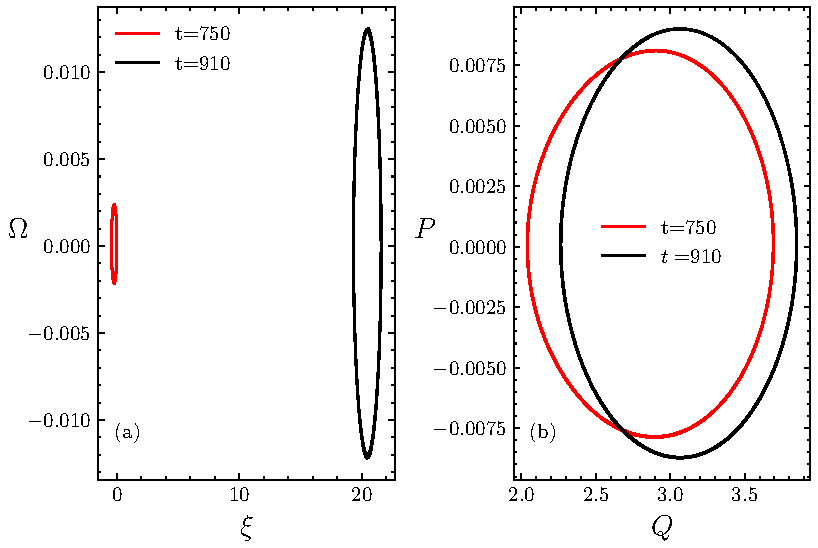
\includegraphics[scale=0.5]{img/area.pdf}
    \caption{Enclosed phase space loop of a particle at different times.
    %at given parameter $a$, $k$ $\omega_{ce}$ etc. 
    \label{fig.area}
    }
\end{figure}
\begin{figure}
    \centering
    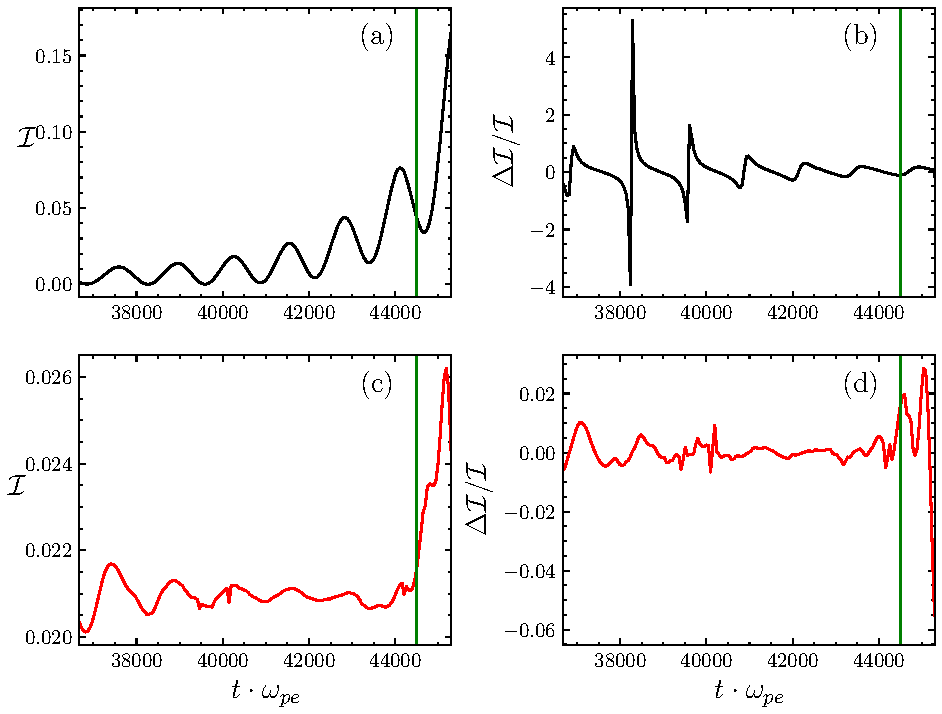
\includegraphics[scale=0.5]{img/adiaI.pdf}
    \caption{Time variation and 
relative change
     of $\mathcal{I}$ of a given particle in the static (the black lines) and  real-time resonance  frames (the red lines).  
     %and (d) shows the relative change of $\mathcal{I}$ with time.(a) and (b) 
    }
    \label{fig.I}
\end{figure}
To quantitatively show the adiabaticity, we numerically calculate the area of the phase loop and show its time variation 
%in Fig. \ref{fig.I}(a) and \ref{fig.I}(c). We also show 
and the relative error of the adiabatic invariant $\mathcal{I}(t)$ in Fig. \ref{fig.I}.
%figure \ref{fig.I} (b) and (d).
Unlike the static frame, the variation of $\mathcal{I}$ is less than $2\%$ in the reference frame following with the resonance,
as seen in Fig. \ref{fig.I}(d). 
The adiabatic invariant $mathcalI$ and the validity of the adiabaticity are shown to be conserved. 
The variation becomes large until the particle approaches the equator, where the wave amplitude is small, and the particle can be released from the wave potential well. 
The releasing of trapped particle, which is reported in the particle in cell (PIC) simulation \cite{tao_trap-release-amplify_2021}, could be a potential reason for the violation of the adiabatic motion.
% \begin{figure}
%     \centering
%     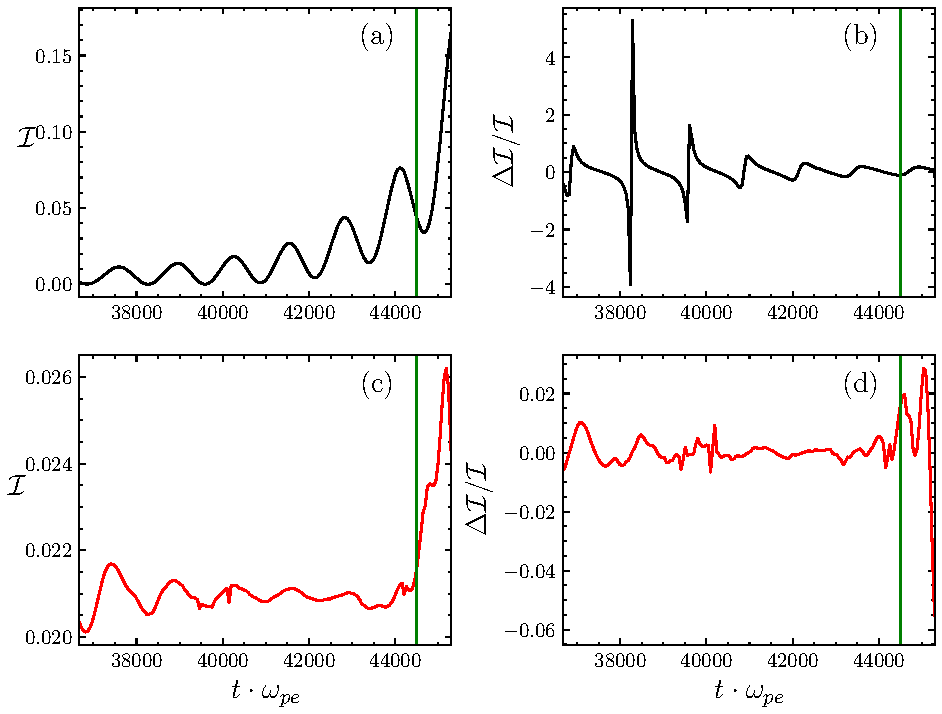
\includegraphics[scale=0.8]{img/adiaI.pdf}
%     \caption{The calculated $\mathcal{I}$ of a given particle in the static frame of reference and the compensated resonance reference.
%     }
%     \label{fig.I}
% \end{figure}

% \begin{figure}
%     \centering
%     \includegraphics[scale=0.8]{img/adiaIR.pdf}
%     \caption{The relative increment of $\mathcal{I}$ for a given particle in the static frame of reference and the compensated resonance reference. 
%     \label{fig.Ierr}
%     }
% \end{figure}
% %\if{1}
% \section{The adiabatic approximation}
%solve current integral and obtain the chirping law
%Nevertheless, harnessing 
With the adiabatic approximation, we can greatly reduce the description of the trapped particle distribution and the energetic particle current.
%In our previous studies, we obtain 
The nonlinear energetic particle current $j_p$ is obtained from the velocity integral of the perturbed distribution function 
\cite{zheng2024}
\begin{equation}\label{eq.ep_current}
    \begin{aligned}
j_p(s_i,t) & = -\frac{1}{ 4 \pi } \frac{\omega_{h0}^2k_i}{e}\iiint \sqrt{2m_e\omega_{ce}(s)(\mathcal{J}+\Omega+\Pi_i)} 
 \\
 &\times f(\xi,\Omega,\mathcal{J};s_i(t),t)e^{\imath \xi} \rm d \xi \rm d \Omega \rm d \mathcal{J}~.
    \end{aligned}
\end{equation}
%The current dominates the nonlinear behavior of the chorus chirping process, and under certain condition, we can simplify the phase space integral and show qualitatively how does the current evolves.
At the nonlinear stage, the distribution function of the trapped electrons forms a hole in phase space.
% and we consider its  $\Delta f$, .
Since the equilibrium distribution does not contribute to the current, the nonlinear current is directly determined by 
the deviation from the unperturbed distribution, i.e., the depth of the hole,
$\Delta f$.
The depth of the hole can be written as the function of the adiabatic invariant, i.e., $\Delta f(s_i,\mathcal{J},\mathcal{I},\xi,t)$.
Now we replace $f$ by $\Delta f$ in the current integral in Eq. (\ref{eq.ep_current}) and write  the integral as
\begin{equation}
\begin{aligned}
    j_p(s_i,t) & \approx - \int\mathrm{d} \mathcal{J} \sqrt{2 \omega_{ce} (\mathcal{J} + \Pi_i(t))}
    \\
    &\times \int_0^{\mathcal{I}_{\mathrm{s p x}}}  \mathrm{d}\mathcal{I}  \oint \mathrm{d}\psi  \Delta f(s_i,\mathcal{J},\mathcal{I},\xi,t)e^{\imath \xi}  ~.
\end{aligned}
\end{equation}
Note that $\Omega$ in the square root has been  neglected since $\Omega \simeq 0$.
The differential area element $\mathrm{d}\xi\mathrm{d}\Omega$ is changed to $\mathrm{d}\mathcal{I}\mathrm{d}\psi$, where $\psi$ is the angle variable of $\mathcal{I}$.
From the Jacobi of the differential element, the integral over $\psi$ is
\begin{equation}
      \oint f \mathrm{d}\psi = \oint f \frac{\mathrm{d}\Omega}{\mathrm{d}\mathcal{I}}\mathrm{d}\xi = \frac{\partial H}{\partial \mathcal{I}} \oint f \frac{\mathrm{d}\Omega}{\mathrm{d} H}\mathrm{d}\xi = \dot{\psi}\oint \frac{f}{\Omega} \mathrm{d}\xi = 2 \pi \langle f \rangle,
\end{equation}
where $\langle\cdots\rangle$ denotes the bounce average, following the definition in Ref. \cite{berk1999}.
Thus the current integral becomes
\begin{equation}\label{eq.adiabatic_current}
\begin{aligned}
    j_p(s_i,t)  &\approx -  {2\pi} \int\mathrm{d} \mathcal{J}  \sqrt{2\omega_{ce} (\mathcal{J} + \Pi_i(t))} \\
    & \times 
    \int_0^{\mathcal{I}_{\mathrm{s p x}}}\mathrm{d}\mathcal{I}  \langle \Delta f(s_i,\mathcal{J},\mathcal{I},\xi,t)e^{\imath \xi} \rangle  ~.
\end{aligned}
\end{equation}
%For the adiabatic regime, the characteristic scales should vary considerably slowly compared to the wave trapping scale.
%There exists a small scale $\epsilon$ satisfies \cite{berk1999}
%\begin{equation}
%    \epsilon \equiv \mathrm{max}\left(\ddot{\omega}/\omega_b^3, \dot{\omega}/\omega_b^2, \omega_b/\omega \right) \ll 1~,
%\end{equation}
%Here, $\omega$ is the frequency deviation from the resonance center in our context.
%For the chorus wave field, the frequency, and other quantities change slowly in one bounce period, satisfying the first and the second inequalities. The last term requires the frequency chirped a notable distance, i.e., the nonlinear stage, where the hole has been separated from the equilibrium.
Note that $\Delta f$ can be expanded in powers of $\epsilon$, a small parameter describing the change of parameters during the bounce motion
%Following  the method in Ref. \cite{berk1999}, 
and the bounce averages in Eq.~(\ref{eq.adiabatic_current}) are 
 \cite{berk1999} 
\begin{equation}
    \begin{aligned}
    \langle\Delta f \sin \xi \rangle &\simeq \alpha \Delta f_0 ~, \\ 
    \langle \Delta f \cos \xi \rangle &\simeq  \Delta f_0 \langle \cos \xi \rangle ~.
    \end{aligned}
\end{equation}
%approximation 2, I is constant over trapped region
We further assume that $\Delta f_0$ is independent of $\mathcal{I}$, which implies that the depth of the hole is flat within the enclosed hole area, i.e., the water bag approximation \cite{omura_theory_2008,hezaveh2021}. 
Therefore, the integral over $\mathcal{I}$ only depend on the $\mathcal{I}_\mathrm{spx}$ which is the 
 adiabatic invariant on the separatrix. 
According to Eq. (\ref{eq.def_I}), we have
\begin{equation}
    \int^{\mathcal{I}_\mathrm{s p x}}_0 \mathrm{d}\mathcal{I} = \mathcal{I}_\mathrm{s p x} \equiv {1\over2\pi} \oint_\mathrm{s p x} \Omega (\xi) \mathrm{d} \xi~,
\end{equation}
where the boundary of the trapped particle phase space hole can be analytically given as
\begin{equation}
    \Omega(\xi) = \pm \frac{\omega_b}{k^2} \sqrt{2 (e_\mathrm{spx}-\cos \xi - \alpha \xi)}~,
\end{equation}
and $e_\mathrm{spx}$ denotes the Hamiltonian on the separatrix.
%, cf. ref. \cite{zheng2023b}.
%Now we define two functions of $\alpha$
Then the current integral becomes  
\begin{equation}\label{eq.adi_J}
    \begin{aligned}
    j_p(s_i,t) & \approx \frac{\sqrt{2} \omega_b}{k^2}  \left(m_\mathrm{s p x}+\imath ~ n_\mathrm{s p x}\right) \\
    & \times  \int \mathrm{d} \mathcal{J} \sqrt{ \omega_{c e}(\mathcal{J}+\Pi_i(t))} \Delta f(\mathcal{J},s_i,t) ~,
    \end{aligned}
\end{equation}
where
\begin{equation}\label{eq.function}
    \begin{aligned}
        m_\mathrm{spx}(\alpha) & = \oint_\mathrm{s p x} \mathrm{d} \xi \cos \xi \sqrt{e_\mathrm{s p x}-\cos \xi-\alpha \xi}, 
        \\
        n_\mathrm{spx}(\alpha) &  = \alpha \oint_\mathrm{s p x} \mathrm{d} \xi \sqrt{e_\mathrm{s p x}-\cos \xi-\alpha \xi}.
    \end{aligned}
\end{equation}
%the nonlinaer currnet and the chirping rate ...
%differnece with omura 
%process approxiamtion strict follows adiabatic approximation
%why the hole is oblique
%alpha value should small to validate approximation
%figure
\begin{figure}
    \centering
    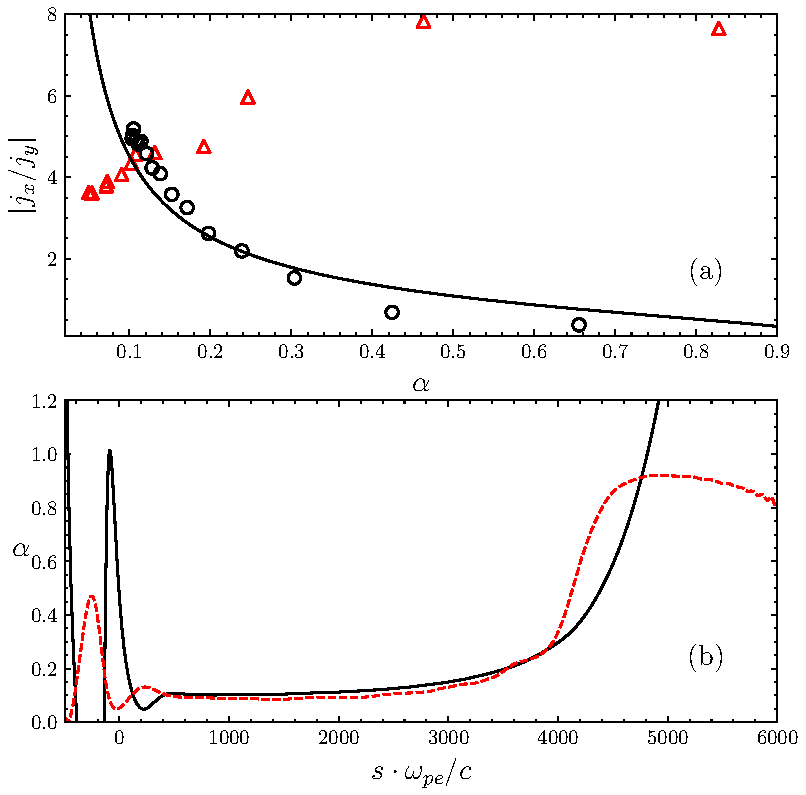
\includegraphics[scale=0.5]{img/alpha.pdf}
    \caption{(a) Current ratio versus the inhomogeneous parameter $\alpha$. The scattered points are obtained at difference spatial locations from the simulation, the triangles are obtained from near the equator region while circus are obtained from the downstream region. 
    The solid curve is the results from adiabatic approximation Eq. (\ref{eq.adia_relation}). 
    (b) Snapshot  of the parameter $\alpha$ at $t = 850$ obtained  from the definition in Eq. (\ref{eq.alpnew}) (black solid line) and  from adiabatic relation (red dashed line).
    }
    \label{fig.adiabatic}
\end{figure}


%A $\delta f$ Vlasov equation coupled with a wave envelope equation are given and self-consistently describes the wave-particle interactions.
%Here, we recall the Vlasov equation for $\delta f(s_i,\vartheta,\mathcal{J},\xi,\Omega)$ 
%\begin{equation}\label{eq.vlasov}
%    \frac{\partial \delta f}{\partial t} + \frac{d s_{i}}{d t} \frac{\partial \delta f}{\partial s_{i}} + \frac{d\mathcal{J}}{dt}\frac{\partial \delta f}{\partial \mathcal{J}} + \frac{\partial \delta f}{\partial \xi}\frac{d \xi}{dt} + \frac{\partial \delta f}{\partial \Omega}\frac{d \Omega}{d t}  = \frac{\partial f_0}{\partial \Omega}\frac{\partial \delta K}{\partial \xi}~,
%\end{equation}
%where $\delta K$ = 
%
%The constant for each cell is determined by the initial choice of $\mathcal{J}$, which give the entire information of the dynamics on the slowly varying scale along the magnetic field line.
%The equations for the fast varying compontens
%\begin{equation}\label{eq.odes2}
%    \begin{aligned}
%    \frac{\mathrm{d}\Omega}{\mathrm{d}t} &= \frac{\omega_b^2}{k_i^2}\left(\sin \xi - \alpha \right)~,
%    \\
%    \frac{\mathrm{d}\xi}{\mathrm{d}t} &= {k_{i}^{2}\Omega}+ \frac{\omega_{ce} }{\sqrt{2\omega_{ce}(\mathcal{J}+\Omega+\Pi_i)}}\frac{e |a|}{c}\cos \xi ~.
%    \end{aligned}
%\end{equation}
%and 
%\begin{equation}\label{eq.alp1}
%   \alpha \simeq \frac{k_l}{\omega_b^2}\left(\mathcal{J}-\frac{\Pi_i}{2}\right) \frac{\partial \omega_{c e}}{\partial s}
%\end{equation}
%
%The wave equation 
%\begin{equation}\label{eq.full}
%    \frac{\partial a}{\partial t} +v_g \frac{\partial a}{\partial s_i} =\frac{-\imath 2\pi v_g}{c k_i } j_p~,
%\end{equation}
%for reference.
%The energetic particle current $j_p$ is
%\begin{equation}\label{eq.ep_current}
%j_p(s_i,t) = -\frac{1}{ 4 \pi } \frac{\omega_{h0}^2k_i}{e}\iiint \sqrt{2m_e\omega_{ce}(s)(\mathcal{J}+\Omega+\Pi_i)} \times f(\xi,\Omega,\mathcal{J};s_i(t),t)e^{\imath \xi} \rm d \xi \rm d \Omega \rm d \mathcal{J}~,
%\end{equation}
The temporospatial evolution of the nonlinear current only depends on the integral over the slowly varying scale $\mathcal{J}$, and an inhomogeneity parameter $\alpha$, defined in Eq. (\ref{eq.alpnew}). 
The $\mathcal{J}$ integral can be calculated further with the adiabatic motion of the trapped particle along the magnetic field line \cite{summers2012}, while the integrals $m_\mathrm{spx}$ and $n_\mathrm{spx}$ can be numerical integrated from Eq. (\ref{eq.function}).
%Since the phase space hole is aligned with the slowly varying wave packet, the hole depth $\Delta f$ also contributes to a complex phase $\delta \phi(s,t)$, which is the phase of the slowly varying wave packet $\delta \phi \equiv \arg(a)$.
Note that, our Vlasov simulation is performed with Hamiltonian Eq. (\ref{eq.H_lab}), thus the phase of the current $j_p$ in the Vlasov simulation also differs $\delta \phi$ with the current relation in Eq. (\ref{eq.adi_J}).
To compared and verify our adiabatic theory, we should also translate this addition phase, i.e., $j^\prime_{p} = j_p \cdot e^{-\imath \delta \phi}$, where $j_p$ is the current from Vlasov equation. 
From Eqs. (\ref{eq.adi_J}) and (\ref{eq.function}), we can find that the ratio of the imaginary and real component of $j^\prime_{p}$ is a function of $\alpha$, 
\begin{equation}\label{eq.adia_relation}
    \begin{aligned}
\frac{j_x}{j_y} &= \frac{\mathrm{real}(j^\prime_p)}{\mathrm{imag}(j^\prime_p)} = \frac{m_\mathrm{spx}}{n_\mathrm{spx}}
\\
& = \frac{\oint_\mathrm{s p x} \mathrm{d} \xi \cos \xi \sqrt{e_\mathrm{s p x}-\cos \xi-\alpha \xi}}{\alpha \oint_\mathrm{s p x} \mathrm{d} \xi \sqrt{e_\mathrm{s p x}-\cos \xi-\alpha \xi}}.
            \end{aligned}
\end{equation}

By numerically solve the integral in above equation, we obtain an explicit relation of current ration with respect to $\alpha$ shown in Fig. \ref{fig.adiabatic}(a). 
Meanwhile, to verify the validity of the relation, we select various spatial locations at $t=850$ from the Vlasov simulation \cite{zheng2023b,zheng2024}, calculate the $\alpha$ from definition in Eq. (\ref{eq.alpnew}), and get the corresponding current ratio.
It is shown that the value obtained in our simulation result well agree with the adiabatic predictions in propagation region of the chorus wave (black circles).
Conversely, the above relation can be applied as an alternative way for evaluating the inhomogeneous parameter $\alpha$ from the energetic particle current, which might be more accurate if the current can be measured somehow.
It is meaningful since the inhomogeneous parameter $\alpha$ is of importance to study the wave-particle interaction and chirping behavior \cite{tao_theoretical_2020,omura2008}.
%The relation provides an alternative way   ,  
%Unlike to the calulating $\alpha$ from the definition, we only need to know the current 

Nevertheless, near the equator region, where the chorus is triggered, (red triangles), the adiabatic approximation is no longer valid.
Similar conclusion can be drawn from the spatial distribution of $\alpha$ calculated from definition in Eq. (\ref{eq.alpnew}) and the adiabatic current relation, as shown in Fig. \ref{fig.adiabatic}(b). 
The evolution of $\alpha$ indicates a rapid variation of the phase space near the equator, which is related to the generation of the nonlinear chorus wave.
The results of nonadiabtic regime also agree with the previous PIC simulations \cite{tao2017a,tao2017b}.


\section{Conclusion}
\label{sec:conc}
In summary, we have explored the dynamics of resonant electrons and the evolution of whistler-mode chorus waves by test particle simulations.
We show that the adiabatic description is valid if one tracks the dynamics in the frame of reference moving the local resonance.
We have derived an analytic current expression and discussed the adiabatic regime in the global domain by showing the wave chirping behavior with respect to the inhomogeneity parameter $\alpha$.
The adiabatic approximation and the reduced current expression reveal the underlying physics for the wave chirping.

\begin{acknowledgments}
    The work was inspired by H.L.Berk during Ge Wang worked with him at the University of Texas.
    As Herb’s former Ph.D. student and long-time collaborator, Ge witnessed Herb’s kindness, diligence, and persistence. Thank you, Herb. 
    This work was supported by the National Natural Science Foundation of China under Grant No.~12275013.
    The simulations were carried out at National Supercomputer Center in Tianjin and  performed on Tianhe new generation supercomputer.
\end{acknowledgments}

%\bibliographystyle{unsrt}
\bibliography{ref.bib}
\end{document}
